\documentclass[tikz]{standalone}
\begin{document}
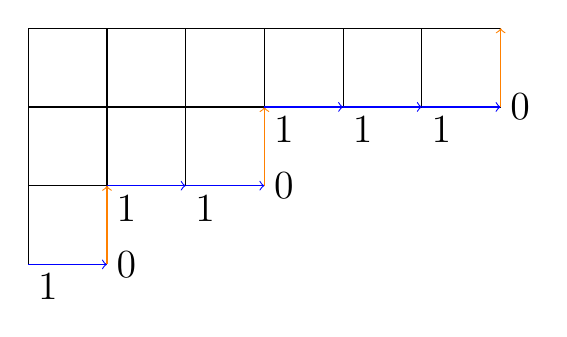
\begin{tikzpicture}
\draw (0,0) -- (6,0);\draw (0,-1) -- (6,-1);\draw (0,-2) -- (3,-2);\draw (0,-3) -- (1,-3);\draw (1,0) -- (1,-3);\draw (2,0) -- (2,-2);\draw (3,0) -- (3,-2);\draw (4,0) -- (4,-1);\draw (5,0) -- (5,-1);\draw (6,0) -- (6,-1);\draw (0,0) -- (0,-3);
\draw[blue, ->] (0,-3) -- (1,-3);\draw[orange, ->] (1,-3) -- (1,-2);\draw[blue, ->] (1,-2) -- (2,-2);\draw[blue, ->] (2,-2) -- (3,-2);\draw[orange, ->] (3,-2) -- (3,-1);\draw[blue, ->] (3,-1) -- (4,-1);\draw[blue, ->] (4,-1) -- (5,-1);\draw[blue, ->] (5,-1) -- (6,-1);\draw[orange, ->] (6,-1) -- (6,-0);
\begin{scope}[font=\Large]
  \draw (0,-3) [below right] node{1};\draw (1,-3) [right] node{0};\draw (1,-2) [below right] node{1};\draw (2,-2) [below right] node{1};\draw (3,-2) [right] node{0};\draw (3,-1) [below right] node{1};\draw (4,-1) [below right] node{1};\draw (5,-1) [below right] node{1};\draw (6,-1) [right] node{0};
\end{scope}
\end{tikzpicture}
\end{document}
